% !TEX program = pdflatex
\documentclass[10pt,a4paper]{article}

% -----------------------
% Encoding + language
% -----------------------
\usepackage[T1]{fontenc}
\usepackage[utf8]{inputenc}
\usepackage[english]{babel}

% -----------------------
% Scalable fonts (fixes pdfTeX microtype expansion issues)
% -----------------------
\usepackage{lmodern}

% -----------------------
% Typography (safe microtype config)
% -----------------------
\usepackage[final]{microtype}
% If your setup still complains, uncomment the next line:
% \microtypesetup{expansion=false}

% -----------------------
% Page layout
% -----------------------
\usepackage{geometry}
\geometry{margin=1.8cm}
\usepackage{subcaption}

\usepackage{setspace}
\onehalfspacing

% -----------------------
% Math + symbols
% -----------------------
\usepackage{amsmath,amssymb}

% -----------------------
% Figures + tables
% -----------------------
\usepackage{graphicx}
\usepackage{float}
\usepackage{booktabs}

% -----------------------
% Links
% -----------------------
\usepackage[hidelinks]{hyperref}

% -----------------------
% Code listings (optional)
% -----------------------
\usepackage{xcolor}
\usepackage{listings}
\lstset{
  basicstyle=\ttfamily\small,
  breaklines=true,
  frame=single,
  columns=fullflexible,
  showstringspaces=false
}

% -----------------------
% Nice lists
% -----------------------
\usepackage{enumitem}
\setlist{noitemsep, topsep=0.3em}

% -----------------------
% Pipeline Visualisation
% -----------------------
\usepackage{tikz}
\usetikzlibrary{arrows.meta, positioning}

% -----------------------
% Title meta
% -----------------------
\title{Radar Visualization Pipeline Report}
\author{Aiysha Mei Frutiger, Sandro Barbazza, Senanur Ates,  \\ University of Basel \\ Computer Architecture}
\date{\today}

\begin{document}
\maketitle

\begin{abstract}
% TODO(Abstract): -> Sandro
%Replace with 150--250 words that state goal + concrete results (e.g., "We successfully ...").
We built a simple ultrasonic ``radar-style'' scanner that measures distance and visualizes the results live in 2D. An Arduino triggers a URM37 ultrasonic sensor, measures the echo pulse width, converts it to centimeters, and sends one newline-terminated record per sample in the format \texttt{angle,cm}. A servo sweeps the sensor so that each reading becomes an \textit{(angle, distance)} pair that can be drawn in polar coordinates on the host.

The system works reliably for typical indoor test objects: stationary targets produce consistent readings across multiple sweeps, and missing or out-of-range echoes are sent as \texttt{-1} and do not create false points in the visualization. Overall, the project shows how sensor measurements can be collected on an Arduino and visualized live on a computer.
\end{abstract}


\tableofcontents
\newpage

% ==========================================================
\section{Introduction}


We built a compact ultrasonic ``radar-style'' scanner that converts echo timing into distance and visualizes it live in 2D.
The servo sweep generates \textit{(angle, distance)} pairs that are transmitted over USB serial and rendered in polar coordinates on the host.



\paragraph{Contributions.}
\begin{itemize}
  \item End-to-end ultrasonic scan pipeline from time-of-flight echo to live 2D visualization.
  \item Arduino firmware for servo sweep, echo-to-distance conversion, and a newline-framed serial protocol.
  \item Processing-based visualization with robust line parsing and bucket-based refresh behavior.
\end{itemize}

% ==========================================================
\section{Methodology}

\subsection{System-level approach}
% TODO(Methodology/System-level): -> Aiysha
%1--2 sentences on *method choices/assumptions* (not implementation details),
% e.g., why ASCII newline framing was chosen (debuggability/simplicity), and what the target behaviour is.
We implement an end-to-end ultrasonic ``radar-style'' pipeline that turns distance measurements into a live 2D visualization.

\paragraph{Pipeline.}
\begin{center}
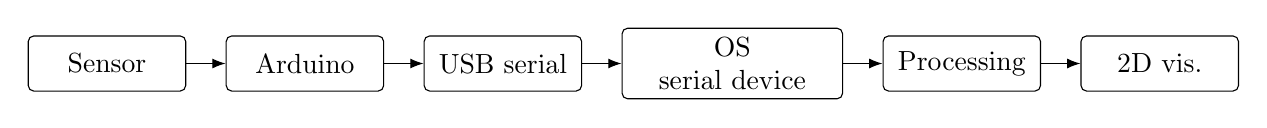
\begin{tikzpicture}[
  box/.style={draw, rounded corners=2pt, minimum height=7mm, minimum width=20mm, align=center},
  arr/.style={-Latex}
]
\node[box] (s) {Sensor};
\node[box, right=5mm of s] (a) {Arduino};
\node[box, right=5mm of a] (u) {USB serial};
\node[box, right=5mm of u, minimum width=28mm] (os) {OS\\serial device};
\node[box, right=5mm of os] (p) {Processing};
\node[box, right=5mm of p] (v) {2D vis.};

\draw[arr] (s) -- (a);
\draw[arr] (a) -- (u);
\draw[arr] (u) -- (os);
\draw[arr] (os) -- (p);
\draw[arr] (p) -- (v);
\end{tikzpicture}
\end{center}

\subsection{Implementation path}
% TODO(Methodology/Implementation path): -> Aiysha/Sena ?
% Optionally add 1 sentence about what exactly was unstable
% (e.g., framing/partial reads/reset timing), and what Processing improved (event-driven reads, line framing).
We first prototyped the UI in C using \texttt{raylib}, but the end-to-end system was unstable on Windows due to low-level serial I/O issues (port selection, reset timing, partial lines, contention). We therefore switched to Processing to simplify serial handling using its line-based, event-driven serial library and to iterate faster.


\subsection{Constraints and iterations}
% TODO(Methodology/Constraints): -> Sandro
% Add 2--4 sentences if relevant:
% - servo unavailable early -> simulated sweep mode
% - any goal changes (range, FOV, etc.)


% ==========================================================
\section{Implementation}

\subsection{Hardware}
% TODO(Implementation/Hardware): -> Sandro
% Add reproducible setup details:
% - components used (Arduino model, ultrasonic sensor model, servo model)
% - wiring summary (pins for trig/echo, servo PWM pin, power)
% - mechanical mount/stand notes (if essential)
% Keep it short but precise.


\subsection{Servo sweep control}
% TODO(Implementation/Servo): -> Sena
% Add concrete parameters and behaviour:
% - angle range (e.g., 15--165), step size (deg), delay between steps
% - PWM library (Servo.h) and how angle is updated
% - how sweep direction changes at boundaries
% (write here)

Sweeping is implemented with \texttt{Servo.h}. The servo moves from \texttt{MIN\_ANGLE} to \texttt{MAX\_ANGLE} in
steps of \texttt{STEP\_ANGLE} and then reverses back.

\paragraph{Parameters.}
\texttt{MIN\_ANGLE=0}, \texttt{MAX\_ANGLE=180}, \texttt{STEP\_ANGLE=2}, \texttt{SERVO\_SETTLE\_MS=30 ms},
\texttt{BETWEEN\_READ\_MS=10 ms}. A settling delay is used before each measurement to reduce motion-related errors.


\subsection{Measurement and serial protocol}
% TODO(Implementation/Measurement): -> Aiysha/Sena ?
% Add missing *exact* conversion and edge cases:
% - formula from echo duration to cm (e.g., t/58 or t/50 depending on sensor mode)
% - timeouts / invalid detection criteria -> when you send -1

% TODO(Implementation/Protocol):  -> Aiysha/Sena ?
% Add missing protocol constants:
% - baud rate (e.g., 9600)
% - exact record format: "angle,cm\n" and value ranges
The ultrasonic sensor returns an \emph{echo pulse width} proportional to time-of-flight. The Arduino triggers the sensor, measures the echo duration (e.g., with \texttt{pulseIn}), converts it to a distance in centimeters, and sends one newline-terminated ASCII record per measurement (\texttt{angle,cm}).

Distance is derived from the URM37 echo pulse width $t$ (in $\mu$s) using:
\[
\text{cm} = \frac{t}{50}.
\]
If \texttt{pulseIn} times out or values are outside sanity bounds, the firmware outputs \texttt{-1}.
Serial runs at \texttt{9600} baud and sends one record per sample as \texttt{angle,cm$\backslash$n}.


\subsection{Host-side data flow}
% TODO(Implementation/Host): -> Aiysha/Sena ?
% Add missing operational details:
% - how the serial port is selected/opened (manual name or auto-detect)
% - how you handle startup garbage/Arduino reset (discard first N lines, wait for "Init", etc.)
Over USB this data is exposed by the OS as a serial device, which Processing reads as a byte stream, frames into lines, parses angle and distance, and uses to update the visualization state.

\paragraph{Pipeline.}
\begin{center}
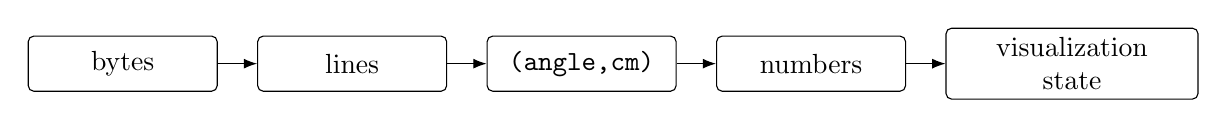
\begin{tikzpicture}[
  box/.style={draw, rounded corners=2pt, minimum height=7mm, minimum width=24mm, align=center},
  arr/.style={-Latex}
]
\node[box] (b) {bytes};
\node[box, right=5mm of b] (l) {lines};
\node[box, right=5mm of l] (t) {\texttt{(angle,cm)}};
\node[box, right=5mm of t] (n) {numbers};
\node[box, right=5mm of n, minimum width=32mm] (st) {visualization\\state};

\draw[arr] (b) -- (l);
\draw[arr] (l) -- (t);
\draw[arr] (t) -- (n);
\draw[arr] (n) -- (st);
\end{tikzpicture}
\end{center}

\subsection{Visualization}
% TODO(Implementation/Visualization): -> Aiysha/Sena ?
% Ensure consistency:
% - In Introduction you mention polar coordinates; here you use 15--165 deg FOV. Make sure this matches servo sweep.

The visualization renders a radar-style scan over a $0^\circ$--$180^\circ$ field of view. A sweep line indicates the current angle, and each incoming $(\textit{angle}, \textit{distance})$ measurement is mapped to polar coordinates to draw a point at the corresponding radius. A static grid (concentric arcs and radial lines) provides scale and orientation.

\subsection{Serial parsing and ``bucket'' state}
% TODO(Implementation/Parsing): -> Aiysha/Sena ?
% Add missing failure handling details:
% - what happens on malformed lines (ignore, log)
% - numeric parsing errors

% TODO(Implementation/Buckets): -> Aiysha/Sena ?
% Add missing parameters:
% - define ANGLE_BUCKET_DEG value
% - how many buckets -> array size and index computation
Processing receives a continuous byte stream and frames it into newline-terminated records. Each line is trimmed, split by comma, and parsed into numeric \textit{angle} and \textit{distance} values; invalid readings are encoded as \texttt{-1} (no detection).

To keep memory bounded and emulate radar refresh behavior, the scan is discretized into fixed-width angle buckets (e.g., \texttt{ANGLE\_BUCKET\_DEG}). Each bucket stores the most recent distance for its slice and is overwritten on the next sweep; a \texttt{-1} clears the corresponding bucket.

Malformed lines or parse errors are ignored. A typical setting is \texttt{ANGLE\_BUCKET\_DEG=2} to match the servo
step size; each bucket stores the latest distance for its angle slice and is overwritten on rescan.



\subsection{Reproducibility notes}
% TODO(Implementation/Repro): -> Aiysha/Sena/Sandro
% Add 4--6 lines to let someone rerun the project:
% - required software versions (Arduino IDE, Processing version)
% - how to flash Arduino, how to start Processing sketch
% - what to configure (COM port name, baud rate)

Flash the Arduino firmware (Arduino IDE 2.x) and verify \texttt{angle,cm} lines at \texttt{9600} baud.
Start the Processing sketch (Processing 4.x), select the correct COM port, and set baud to \texttt{9600}.
The full code and assets are in the GitHub repository referenced below.



% ==========================================================
\section{Evaluation}

\subsection{Functional validation}
% TODO(Evaluation/Functional): -> Sandro
% Report what you tested and what worked:
% - live updates, correct sweep behaviour, object detection, -1 clears, etc.
% - include 2--4 concrete observations

\subsection{Performance and limitations}
% TODO(Evaluation/Performance): -> Sandro
% Add a few measurable or at least observable metrics:
% - max reliable distance (approx.)
% - update rate (measurements per second or sweep time)
% - angular resolution (servo step)

% TODO(Evaluation/Limitations): -> Sandro
% Briefly note known limitations (surface angle, noise, servo backlash).


\subsection{Match with project goals}
% TODO(Evaluation/Goals): -> Sandro
% 2--3 sentences: did you meet original goal, what remains incomplete, why.


% ==========================================================
\section{Conclusion}
We built an end-to-end ultrasonic ``radar-style'' system that converts echo time-of-flight into a live 2D visualization. The stack is observable from Arduino signal processing and USB serial transport to host-side parsing and rendering in Processing.

A key lesson was robustness across layers: we addressed practical serial-port issues (exclusive access, startup noise) and supported both simulated sweep mode (when the servo was unavailable) and real-angle mode when angle data is present.

\paragraph{Self-assessment and outlook.}
We kept the project intentionally simple to understand each layer of the pipeline. With more time, we would increase complexity by adding an on-device LCD (instead of a PC-based UI) and basic controls such as a power switch and calibration routine.

\paragraph{Division of labor.}
All group members assembled the hardware setup and testing. Sandro implemented the main Arduino sensing/communication code and built the stand/chassis. Senanur developed the Arduino servo sweep control. Aiysha implemented the Processing visualization, including parsing and bucket-based rendering.

% ==========================================================
\newpage
\section*{References}
\addcontentsline{toc}{section}{References}

\begin{itemize}
  \item Processing (project homepage + downloads): \url{https://processing.org/} \url{https://processing.org/download/} % :contentReference[oaicite:0]{index=0}
  \item Processing Serial library reference (Serial class): \url{https://processing.org/reference/libraries/serial/Serial.html} % :contentReference[oaicite:1]{index=1}
  \item Processing Serial library reference (bufferUntil): \url{https://processing.org/reference/libraries/serial/Serial_bufferUntil_.html} % :contentReference[oaicite:2]{index=2}
  \item Processing Serial library reference (readStringUntil — common alternative used with newline framing): \url{https://processing.org/reference/libraries/serial/Serial_readStringUntil_.html} % :contentReference[oaicite:3]{index=3}
  \item Processing Serial library reference (serialEvent): \url{https://processing.org/reference/libraries/serial/serialEvent_.html} % :contentReference[oaicite:4]{index=4}
  \item Project source code repository: \url{https://github.com/ateschsena/Radar.git}
\end{itemize}

%==========================================================
\section*{Declaration of Authorship}
\addcontentsline{toc}{section}{Declaration of Authorship}

ChatGPT was used solely to improve the clarity and coherence of the report's language. All ideas, analyses, 
and interpretations presented reflect the group's own work and research.

\end{document}
